\chapter{Implementation}
\label{chap:implementation}
This chapter will detail the development and implementation of the automation
platform as well as the configuration of \gls{aci} and vCenter
\section{ACI Configuration}
The initial wizard was used to set up the fabric and bring it up to a level
where configuration can be applied. During the wizard, the first thing to
configure is the fabric membership, where the auto-discovered spines and leafs
are onboarded and registered into \gls{apic}.
One of the most important settings is to configure the spine to perform as a
BGP route reflector, this is because \gls{mp-bgp} is used internally inside of
\gls{aci} to advertise routes. Figure \ref{fig:bgp-reflection} shows how
\gls{as} 65001 was chosen.

\begin{figure}[H]

    \centering
    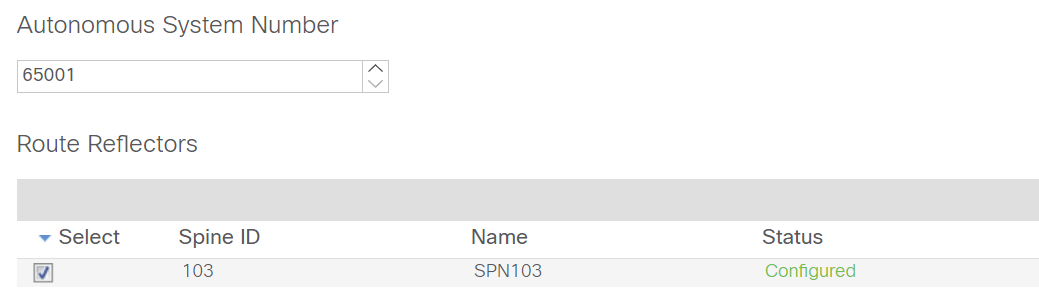
\includegraphics[scale=0.5]{images/bgp-reflection.png}

    \caption{BGP Route Relfection}
    \label{fig:bgp-reflection}
\end{figure}

Other settings such as \gls{dns} and \gls{ntp} were configured to ensure that
all devices have name resolution and that all clocks are in sync.
\gls{oob} IP addresses were also configured so that the fabric nodes can be
reached via \gls{ssh} for troubleshooting purposes, figure \ref{fig:aci-oob-ip}
shows the configuration of the \gls{oob} IP addresses.

\begin{figure}[H]

    \centering
    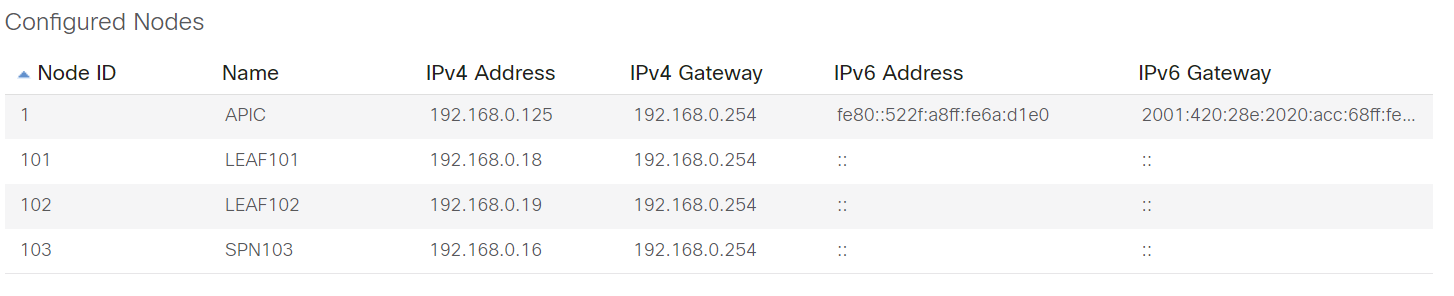
\includegraphics[scale=0.5]{images/aci-oob-ip.png}

    \caption{ACI Out of Band IP Configuration}
    \label{fig:aci-oob-ip}
\end{figure}

\subsection{VMware vCenter Integration with ACI}
\gls{aci} provides the handy functionality of being able to integrate with
vCenter and automatically push created \gls{epg}s into vCenter in the form of
\gls{dpg}s with the VLAN tagging being handled automatically.
Firstly, a dynamic VLAN pool was created which is required so that VLANs can
automatically be associated with \gls{epg}s and \gls{dpg}s. Figure
\ref{fig:vmm-integration} shows the configuration of the VMWare integration.

\begin{figure}[H]

    \centering
    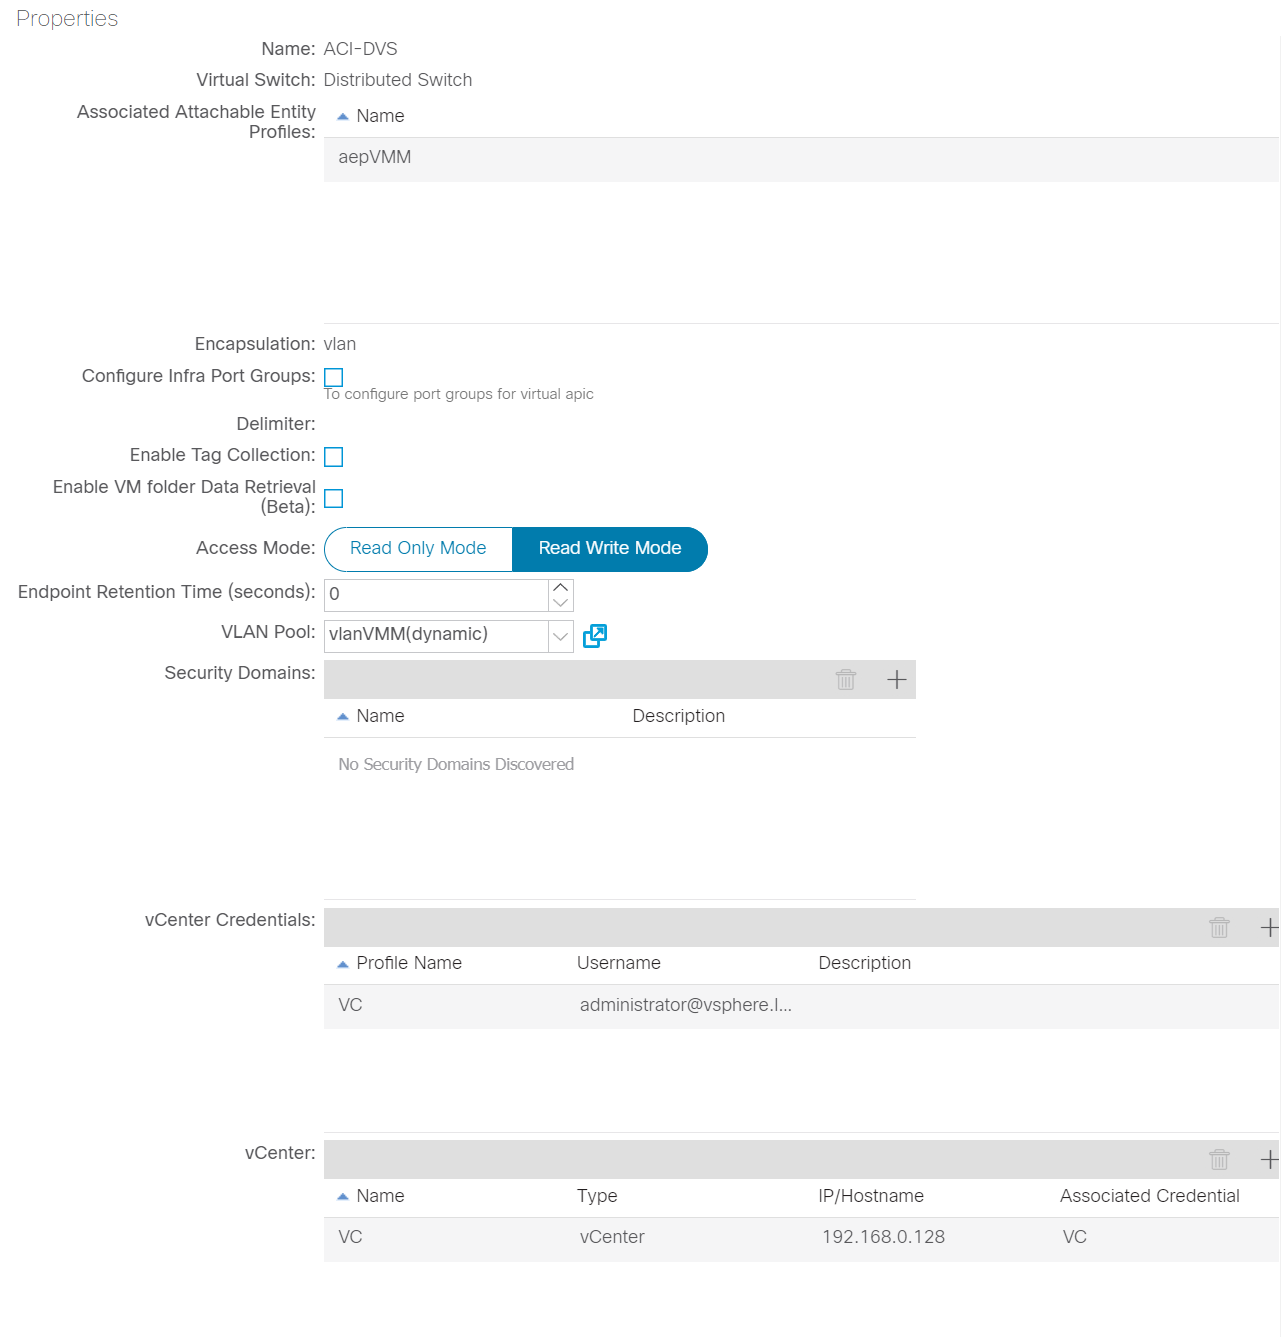
\includegraphics[scale=0.6]{images/vmm-integration.png}

    \caption{VMWare Integration Configuration}
    \label{fig:vmm-integration}
\end{figure}

To get the dual-homed connection of the ESXi host to the two leafs operational,
the two leafs must be brought together to form a \gls{vpc} pair.
Firstly, a \gls{vpc} protection group must be created to inform \gls{aci} that
these two leafs should have a keepalive link formed via the spine between them.
\begin{figure}[H]

    \centering
    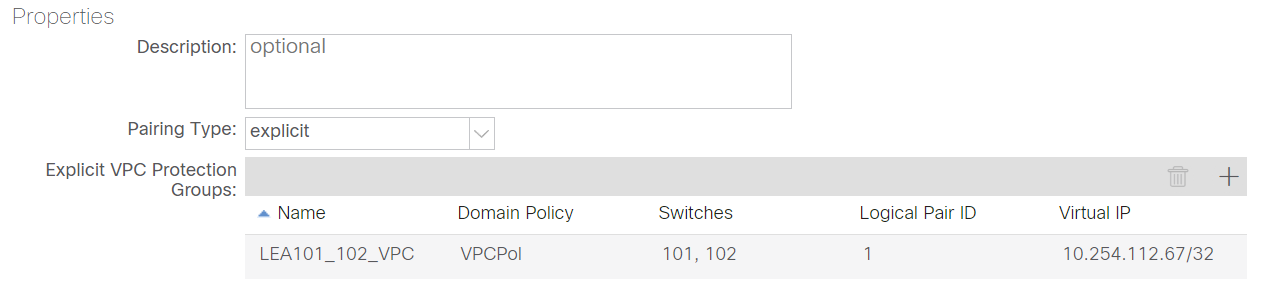
\includegraphics[scale=0.7]{images/vpc-protection.png}

    \caption{vPC Protection Group}
    \label{fig:vpc-protection}
\end{figure}

A \gls{vpc} policy group can then be created to associate the VMWare
integration with the \gls{aaep}, and to also configure the interfaces
associated with the group to use LACP.

\begin{figure}[H]

    \centering
    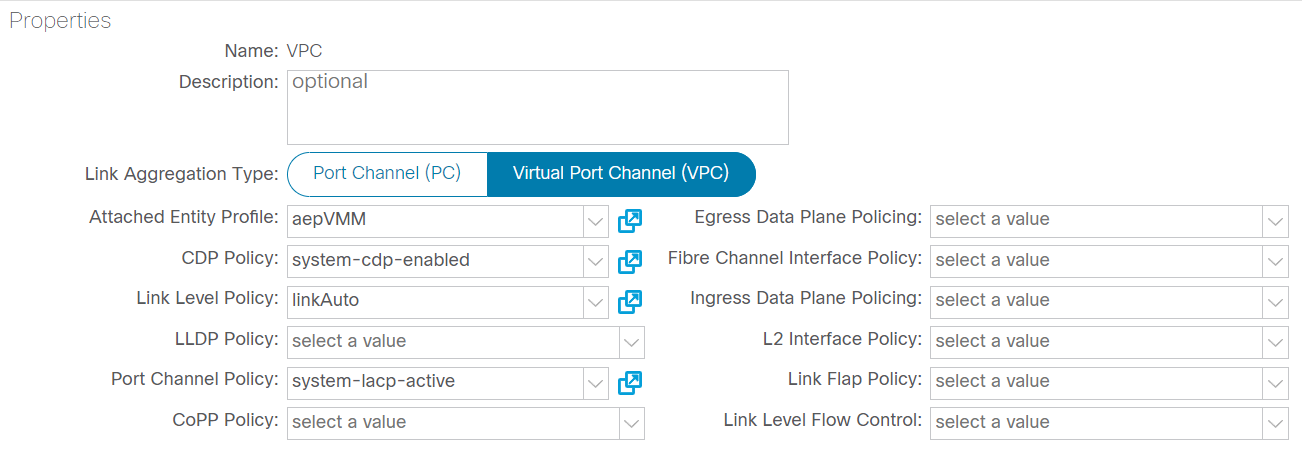
\includegraphics[scale=0.7]{images/vpc-interface-policy.png}

    \caption{vPC Interface Policy Group}
    \label{fig:vpc-int-pol}
\end{figure}

This \gls{vpc} policy group can then be applied to the interfaces on the leafs
via an interface profile which is shown in figure
\ref{fig:vpc-interface-assignment}.
\begin{figure}[H]

    \centering
    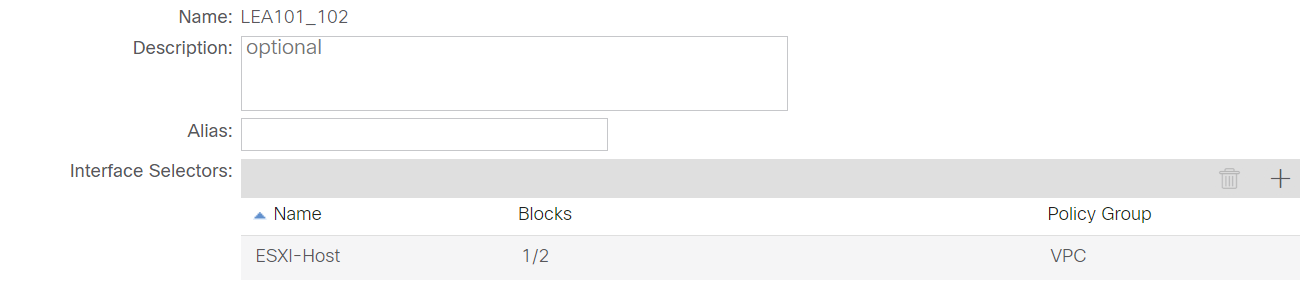
\includegraphics[scale=0.7]{images/vpc-interface-assignment.png}

    \caption{vPC Interface Assignment}
    \label{fig:vpc-interface-assignment}
\end{figure}

In vCenter, figure \ref{fig:vcenter-dvs} shows that \gls{aci} has correctly
pushed the \gls{dvs} to vCenter.

\begin{figure}[H]

    \centering
    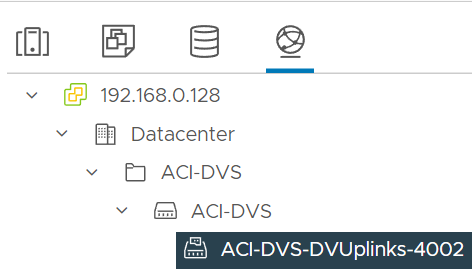
\includegraphics[scale=0.7]{images/vcenter-dvs.png}

    \caption{vCenter Distributed Virtual Switch}
    \label{fig:vcenter-dvs}
\end{figure}
Now the uplinks need to be assigned to the \gls{lacp} group that has been
created by ACI. Figure \ref{fig:uplink-lacp} shows the configuration of the
uplinks to use LACP.

\begin{figure}[H]

    \centering
    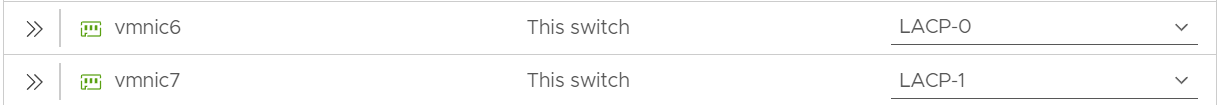
\includegraphics[scale=0.7]{images/lacp-interface-assignment.png}

    \caption{Uplink LACP Configuration}
    \label{fig:uplink-lacp}
\end{figure}
The command \verb|fab 101 show vpc extended| can then be executed on the \gls{apic} via \gls{ssh} to retrieve the status of all \gls{vpc} present on leaf 101.
\begin{figure}[H]
\begin{small}
    \begin{verbatim}
    vPC status
-----------------------------------------------------------------------------
id   Port   Status Consistency Reason      Active vlans         Bndl Grp Name
--   ----   ------ ----------- ------      -------------------- -------------
343  Po3    up     success     success     1135,1168-1169,1200- VPC
                                            1201

    \end{verbatim}
\end{small}
\caption{vPC Status on Leaf 101}
\label{fig:vpc-status}
\end{figure}


\subsection{TEN\textunderscore INFRA Tenant Setup}
With vCenter integration complete, the tenant can now be created that will house all policies related to the infrastructure of the testbed. All of the \gls{vrf}s/\gls{bd}s/\gls{epg}s were created in accordance with the topology shown in figure \ref{fig:epg-topology}.

To get external connectivity working with the \gls{nat} router that will be provisioned inside vCenter, L3Out configuration must be created. Figure \ref{fig:l3out} shows the configuration of the L3Out that will be used for the Infra \gls{vrf}, an \gls{ospf} area of 1 has been specified. A floating \gls{svi} has been utilised so that the VMWare integration configured earlier can be used to pass the L3out \gls{epg} to vCenter automatically. A new static VLAN pool was created along with a new L3 domain. This L3 domain was then added to the VMWare integration so that L3Outs can then use the VMWare virtual domain.

\begin{figure}[H]

    \centering
    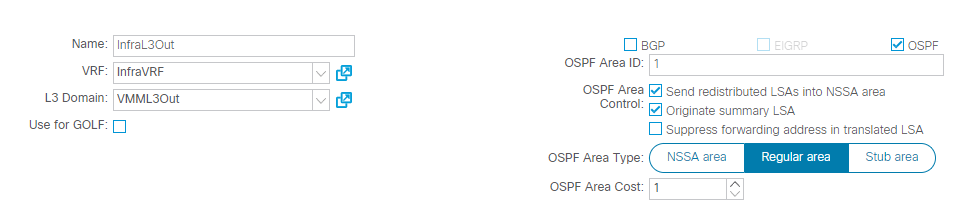
\includegraphics[scale=0.6]{images/InfraL3Out.png}

    \caption{Infra L3Out Configuration}
    \label{fig:l3out}
\end{figure}

\begin{figure}[H]

    \centering
    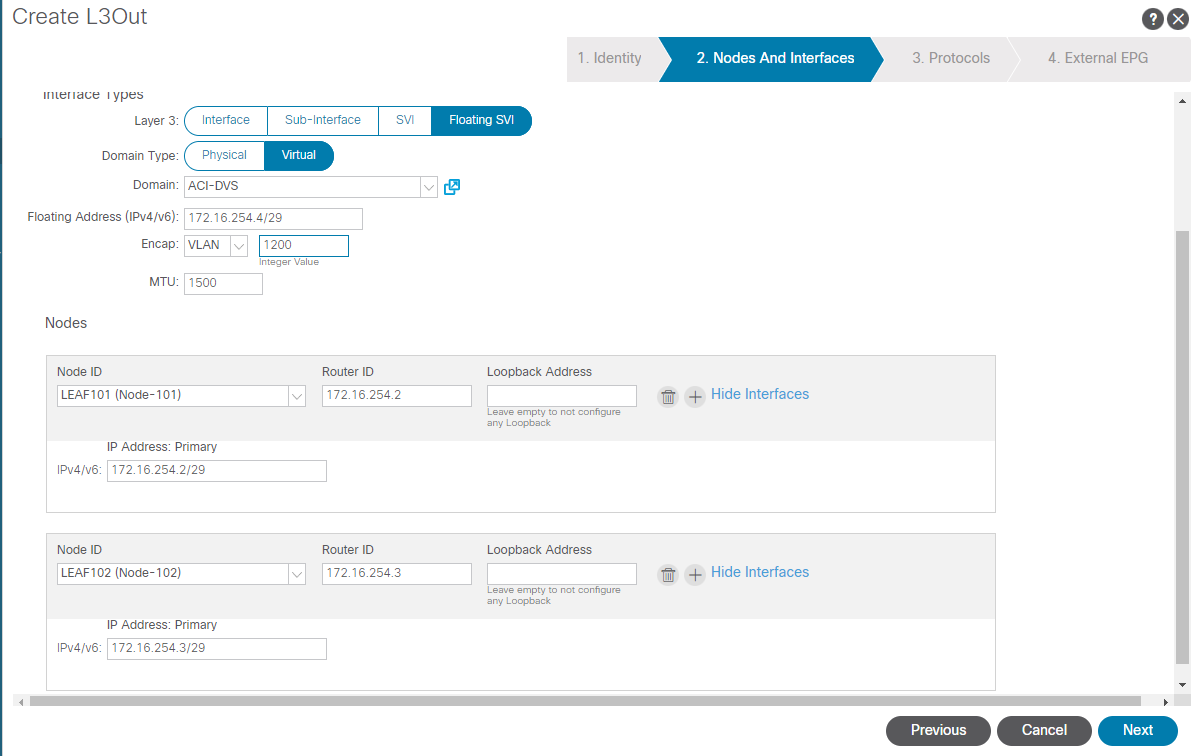
\includegraphics[scale=0.47]{images/InfraL3OutNodes.png}

    \caption{Adding the leafs to the L3Out}
    \label{fig:l3out-nodes}
\end{figure}

It is then important to assign the L3out interface profiles to the enhanced \gls{lacp} group so that the OSPF and traffic flow utilise \gls{lacp} to vCenter correctly. Figure \ref{fig:l3out-lacp} shows the configuration of the L3Out interface profiles.

\begin{figure}[H]

    \centering
    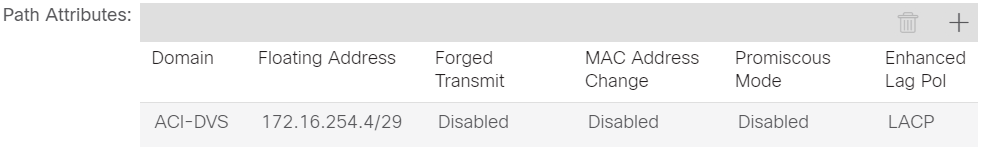
\includegraphics[scale=0.8]{images/l3out-lacp.png}

    \caption{L3Out Interface Profile Configuration}
    \label{fig:l3out-lacp}
\end{figure}

The same process will be repeated for the InternetL3Out for the InternetVRF.

The \gls{nat} router can then be deployed and attached to the L3Out \gls{epg}s via the \gls{dpg}s that have been pushed to vCenter by \gls{aci}.

\subsubsection{NAT Router Configuration}

For virtual routing, the Cisco CSR1000v Virtual Router was chosen. The interfaces were configured with IP addresses that are present in the subnets that were used in the earlier L3Out configuration. \gls{ospf} was also configured so that the routes to and from \gls{aci} are advertised correctly. The following \gls{ospf} configuration was used for the \gls{nat} router.

\begin{figure}[H]
    \begin{verbatim}
        router ospf 1
        passive-interface default
        no passive-interface GigabitEthernet1
        network 172.16.254.0 0.0.0.7 area 1
        default-information originate
        !
        router ospf 2
        passive-interface default
        no passive-interface GigabitEthernet2
        network 172.16.254.8 0.0.0.7 area 2
        default-information originate
    \end{verbatim}
\caption{NAT Router OSPF Configuration}
\label{fig:nat-ospf}
\end{figure}

To verify the \gls{ospf} configuration is working correctly, the following command and output was executed on the \gls{nat} router.

\begin{figure}[H]
    \centering
    \begin{small}
    \begin{verbatim}
InternetRouter#show ip ospf neighbor

Neighbor ID    Pri  State      Dead Time   Address         Interface
172.16.254.10    1  FULL/BDR   00:00:35    172.16.254.10   GigabitEthernet2
172.16.254.11    1  FULL/DR    00:00:33    172.16.254.11   GigabitEthernet2
172.16.254.2     1  FULL/BDR   00:00:39    172.16.254.2    GigabitEthernet1
172.16.254.3     1  FULL/DR    00:00:32    172.16.254.3    GigabitEthernet1

    \end{verbatim}
\end{small}
\caption{NAT Router OSPF Neighbors}
\label{fig:nat-ospf-db}
\end{figure}

Basic \gls{nat} overload can then be configured for all subnets present on \gls{aci} so that the various bridge domains now have internet via the router.

